\pdfoutput=1
\documentclass[11pt]{article}

% --- Packages ---
\usepackage[utf8]{inputenc}
\usepackage[T1]{fontenc}
\usepackage{amsmath,amssymb,amsthm}
\usepackage{graphicx}
\usepackage{booktabs}
\usepackage{array}
\usepackage{tabularx}
\usepackage{multirow}
\usepackage{url}
\usepackage[numbers]{natbib}
\usepackage{xcolor}
\usepackage{tikz}
\usetikzlibrary{arrows.meta,positioning,fit,backgrounds,shapes.geometric,calc}
\usepackage[margin=1in]{geometry}
\usepackage{hyperref}
\hypersetup{
  colorlinks=true,
  linkcolor=blue!60!black,
  citecolor=blue!60!black,
  urlcolor=blue!60!black
}

% --- Theorem environments ---
\newtheorem{theorem}{Theorem}
\newtheorem{corollary}[theorem]{Corollary}
\newtheorem{definition}{Definition}

% --- Title ---
\title{\textbf{GHOST\_DOMAIN}: Semantic Camouflage for\\Privacy-Preserving LLM Interaction\\via Virtual Domain Construction}

\author{
  Myeong Jun Jo\\
  ANIMA Research, Independent Researcher, South Korea\\
  ORCID: \href{https://orcid.org/0009-0006-9540-4666}{0009-0006-9540-4666}
}

\date{}

\begin{document}
\maketitle

% ============================================================
% ABSTRACT
% ============================================================
\begin{abstract}
Enterprises face a fundamental tension: commercial large language models (LLMs) deliver transformative analytical capabilities, but using them requires transmitting sensitive data to external services. We present \textsc{Ghost\_Domain}, a 5-layer semantic camouflage system that resolves this tension by substituting the entire domain of the original data with a semantically disjoint virtual domain---e.g., semiconductor process parameters become musical instrument tuning data---while preserving the topological structure of entity relationships. The LLM performs analytically equivalent reasoning on the camouflaged input, and results are losslessly restored to the original domain via inverse mapping. We formalize security guarantees using information-theoretic bounds: under equivalence class partitioning with parameter~$K$, the conditional entropy satisfies $H(S|O) \geq \log_2(N/K)$ and the recovery probability is bounded by $P(\text{recovery}) \leq K/N$, independent of the number of observations collected by any adversary---including Bayesian-optimal and collusion attackers. Empirical validation across 18 independent experiments confirms round-trip accuracy of 1.000, frequency analysis top-1 advantage $\leq 0.035$, and structural fingerprint recovery that decays as $O(\log N / N)$. \textsc{Ghost\_Domain} provides quantitative, information-theoretic privacy guarantees for a problem that existing techniques---keyword filtering, data masking, on-premise deployment---address only heuristically or at prohibitive cost.
\end{abstract}

\noindent\textbf{Keywords:} LLM privacy, semantic camouflage, data protection, information-theoretic security, domain substitution, cognitive path confinement

% ============================================================
% 1. INTRODUCTION
% ============================================================
\section{Introduction}

The rapid adoption of commercial large language models (LLMs) such as GPT-4~\cite{openai2023gpt4}, Claude~\cite{anthropic2024claude}, and Gemini~\cite{google2024gemini} has created a fundamental tension between productivity and data security. Organizations recognize the analytical power of these models for document analysis, code generation, and decision support, yet transmitting sensitive data to external LLM services exposes proprietary information to potential leakage.

The severity of this risk is well-documented. In 2023, a Samsung semiconductor employee inadvertently uploaded source code and meeting notes to ChatGPT, prompting numerous enterprises---including JP Morgan, Apple, and Amazon---to ban or severely restrict external LLM usage. This represents a costly trade-off: organizations either forfeit the productivity gains of state-of-the-art LLMs or accept uncontrolled data exposure.

The threat is not hypothetical. Carlini et al.~\cite{carlini2021extracting} demonstrated that LLMs memorize and can be prompted to regurgitate training data, establishing that data sent to LLMs is not merely ``processed'' but potentially retained and extractable. More recently, prompt leaking attacks~\cite{hui2024pleak} have shown that even system prompts---supposedly hidden from users---can be systematically extracted from production LLM applications. Membership inference attacks against fine-tuned LLMs~\cite{duan2024membership,fu2024membership} further demonstrate that adversaries can determine whether specific data was used in model training, raising concerns about data exposure even in ostensibly private fine-tuning pipelines.

Existing mitigation strategies are fundamentally limited:

\begin{enumerate}
\item \textbf{On-premise LLM deployment} eliminates data leakage but requires hundreds of millions in infrastructure investment, with model quality significantly lagging commercial offerings. This option is infeasible for small and medium enterprises.

\item \textbf{Data Loss Prevention (DLP) filtering} relies on keyword matching, which is trivially bypassed through paraphrasing and fails to detect contextual sensitivity. The sentence ``raising temperature by 5 degrees increases oxide thickness by 3nm'' contains no flagged keywords but reveals critical semiconductor process parameters.

\item \textbf{Data masking and anonymization} introduces information loss that degrades LLM analysis quality. Simple pseudonymization preserves relational patterns that enable re-identification through frequency analysis across sessions.
\end{enumerate}

We propose a fundamentally different approach. Rather than hiding parts of the data (masking) or blocking keywords (DLP), \textsc{Ghost\_Domain} substitutes the entire domain---entities, relationships, terminology, and context---with a semantically disjoint virtual domain while preserving the topological structure of entity relationships. The LLM operates entirely within the virtual domain, producing analytically equivalent results that are losslessly restored to the original domain through inverse mapping.

The core insight is simple: if a server overload problem is presented as an oven overheating problem, the LLM's causal reasoning is identical---``reduce simultaneous high-load operations and distribute across backup units''---but no server-related information ever leaves the enterprise perimeter.

\paragraph{Contributions.}
\begin{enumerate}
\item We introduce a \textbf{5-layer protection architecture} (Section~\ref{sec:architecture}) that integrates semantic mapping, dynamic domain rotation, metadata isolation, cognitive path confinement, and verified reverse restoration.

\item We formalize \textbf{information-theoretic security guarantees} (Section~\ref{sec:security}) with proof sketches based on equivalence class partitioning, providing $H(S|O) \geq \log_2(N/K)$ conditional entropy and $P(\text{recovery}) \leq K/N$ recovery bounds that hold against Bayesian-optimal and collusion adversaries, independent of the number of observations.

\item We report \textbf{empirical validation} (Section~\ref{sec:experiments}) across 18 independent experiments demonstrating round-trip accuracy of 1.000, quantified resistance to six distinct threat models, and analysis quality of 97--100\% relative to direct (unprotected) LLM analysis, measured via task-specific accuracy metrics.

\item We identify and defend against \textbf{seven specific threat models} (Section~\ref{sec:threats}), including a previously undocumented threat---LLM meta-reasoning attacks where the model itself attempts to infer the original domain from semantic inconsistencies in the camouflaged input.
\end{enumerate}

% ============================================================
% 2. RELATED WORK
% ============================================================
\section{Related Work}

\subsection{Differential Privacy}
Differential privacy (DP)~\cite{dwork2006calibrating} provides formal privacy guarantees by adding calibrated noise to query outputs. While DP offers strong theoretical foundations, it operates on output perturbation rather than input transformation. In the LLM interaction setting, the sensitive data must still be transmitted to the model; DP protects what the model reveals, not what it receives. \textsc{Ghost\_Domain} is complementary: it ensures the model never receives the original data in any form. R\'enyi differential privacy~\cite{mironov2017renyi} provides tighter composition bounds but shares the same fundamental limitation of operating on the output side.

\subsection{Federated Learning and Secure Computation}
Federated learning~\cite{mcmahan2017communication} and secure multi-party computation~\cite{yao1986generate} enable model training or inference without raw data exchange. However, these approaches require architectural cooperation from the LLM provider---custom training pipelines, encrypted inference protocols---which commercial API-based services do not support. \textsc{Ghost\_Domain} operates as a client-side middleware requiring no modification to the LLM service.

\subsection{Prompt Protection and Text Sanitization}
Recent work on prompt injection defense~\cite{perez2022ignore} focuses on protecting the LLM from malicious inputs, not protecting user data from the LLM. Text anonymization tools~\cite{lison2021anonymisation} perform named entity recognition and replacement but do not preserve the semantic structure needed for analytical reasoning, resulting in degraded output quality.

\subsection{LLM-Specific Privacy Threats}
The privacy risks of LLM interaction extend beyond training data memorization. Carlini et al.~\cite{carlini2021extracting} demonstrated that LLMs can be prompted to regurgitate verbatim training data, establishing that data sent to LLMs is potentially retained and extractable. Hui et al.~\cite{hui2024pleak} introduced PLeak, a systematic framework for extracting system prompts from production LLM applications, showing that even hidden instructions can be recovered through optimized adversarial queries. Duan et al.~\cite{duan2024membership} performed a large-scale evaluation of membership inference attacks (MIAs) on LLMs trained on the Pile, finding that while MIAs on pre-training data are difficult, specific distribution-shift settings create exploitable vulnerabilities. Fu et al.~\cite{fu2024membership} further demonstrated that fine-tuned LLMs are significantly more vulnerable, achieving AUC $> 0.9$ through self-prompt calibration techniques. These findings collectively establish that data transmitted to LLM services faces multiple vectors of compromise---memorization, extraction, and inference---motivating the need for input-side protection rather than relying solely on provider-side safeguards.

\subsection{Data Anonymization}
Classical anonymization techniques---$k$-anonymity~\cite{sweeney2002kanonymity}, $l$-diversity, $t$-closeness~\cite{li2007tcloseness}---were designed for tabular data release. They do not address the challenge of preserving analytical utility for natural language processing tasks, nor do they provide guarantees against an adversary who observes multiple anonymized versions of the same dataset across sessions. Narayanan and Shmatikov~\cite{narayanan2008robust} demonstrated that na\"ive anonymization of large sparse datasets is trivially reversible through cross-referencing, motivating the need for information-theoretically grounded defenses.

\subsection{Distinction of GHOST\_DOMAIN}
Our approach differs from all of the above in three fundamental ways: (1) it operates on domain-level substitution rather than entity-level masking, preserving the full relational topology; (2) it provides information-theoretic security bounds that hold against adaptive, multi-session adversaries; and (3) it requires no cooperation from the LLM provider, functioning as a transparent client-side layer.

% ============================================================
% 3. SYSTEM ARCHITECTURE
% ============================================================
\section{System Architecture}
\label{sec:architecture}

\textsc{Ghost\_Domain} consists of five layers, each addressing a distinct aspect of the data protection pipeline. Figure~\ref{fig:architecture} illustrates the system architecture.

% --- Figure 1: System Architecture ---
\begin{figure}[t]
\centering
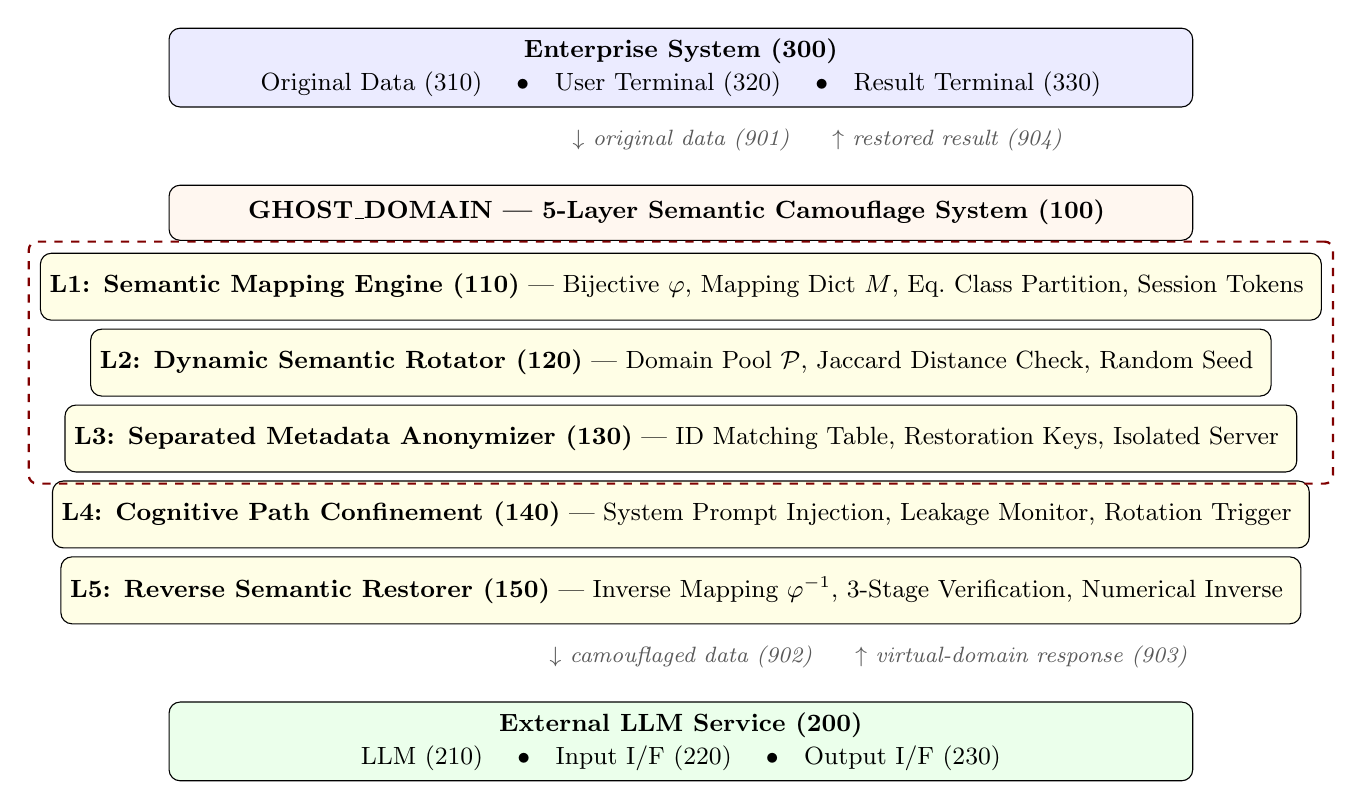
\begin{tikzpicture}[
  node distance=0.4cm,
  layer/.style={draw, rounded corners=4pt, minimum width=13cm, minimum height=0.85cm, font=\small, align=center},
  block/.style={draw, rounded corners=4pt, minimum width=4cm, minimum height=0.7cm, font=\small, fill=white},
  arrow/.style={-{Stealth[length=3mm]}, thick},
  label/.style={font=\footnotesize\itshape, text=gray!70!black},
]

% Enterprise System (top)
\node[layer, fill=blue!8, minimum height=1.0cm] (enterprise) {
  \textbf{Enterprise System (300)}\\[1pt]
  Original Data (310) \quad$\bullet$\quad User Terminal (320) \quad$\bullet$\quad Result Terminal (330)
};

% Flow label: original data
\node[label, below=0.15cm of enterprise] (flow1) {$\downarrow$ original data (901)};

% GHOST_DOMAIN 5-Layer System
\node[layer, fill=orange!6, below=0.3cm of flow1, minimum height=0.7cm] (gd_title) {
  \textbf{GHOST\_DOMAIN --- 5-Layer Semantic Camouflage System (100)}
};

\node[layer, fill=yellow!10, below=0.15cm of gd_title] (l1) {
  \textbf{L1: Semantic Mapping Engine (110)} --- Bijective $\varphi$, Mapping Dict $M$, Eq.\ Class Partition, Session Tokens
};

\node[layer, fill=yellow!10, below=0.1cm of l1] (l2) {
  \textbf{L2: Dynamic Semantic Rotator (120)} --- Domain Pool $\mathcal{P}$, Jaccard Distance Check, Random Seed
};

\node[layer, fill=yellow!10, below=0.1cm of l2] (l3) {
  \textbf{L3: Separated Metadata Anonymizer (130)} --- ID Matching Table, Restoration Keys, Isolated Server
};

\node[layer, fill=yellow!10, below=0.1cm of l3] (l4) {
  \textbf{L4: Cognitive Path Confinement (140)} --- System Prompt Injection, Leakage Monitor, Rotation Trigger
};

\node[layer, fill=yellow!10, below=0.1cm of l4] (l5) {
  \textbf{L5: Reverse Semantic Restorer (150)} --- Inverse Mapping $\varphi^{-1}$, 3-Stage Verification, Numerical Inverse
};

% Flow label: camouflaged data
\node[label, below=0.15cm of l5] (flow2) {$\downarrow$ camouflaged data (902)};

% External LLM Service
\node[layer, fill=green!8, below=0.3cm of flow2, minimum height=1.0cm] (llm) {
  \textbf{External LLM Service (200)}\\[1pt]
  LLM (210) \quad$\bullet$\quad Input I/F (220) \quad$\bullet$\quad Output I/F (230)
};

% Return arrows (right side)
\node[label, right=0.3cm of flow2, anchor=west] (flow3) {$\uparrow$ virtual-domain response (903)};

\node[label, right=0.3cm of flow1, anchor=west] (flow4) {$\uparrow$ restored result (904)};

% Dashed boundary for mapping dict
\node[draw, dashed, thick, red!50!black, rounded corners=3pt,
  fit=(l1)(l3), inner sep=4pt, label={[font=\tiny, red!50!black]right:Mapping Dict \& Keys (905) --- never leave enterprise}] {};

\end{tikzpicture}
\caption{\textsc{Ghost\_Domain} system architecture. Original data flows from the enterprise system through 5 protection layers before reaching the external LLM. The LLM's response traverses the reverse path for restoration. The mapping dictionary and restoration keys (dashed boundary, 905) never leave the enterprise perimeter.}
\label{fig:architecture}
\end{figure}


\subsection{Layer 1: Semantic Mapping Engine}
The core of \textsc{Ghost\_Domain} is a bijective mapping function that transforms the original domain into a virtual domain while preserving relational topology.

\begin{definition}[Domain Topology]
The original domain $\mathcal{D}_O$ is represented as a directed graph $G_O = (E_O, R_O)$ where $E_O = \{e_1, e_2, \ldots, e_n\}$ is the entity set and $R_O = \{r_1, r_2, \ldots, r_m\}$ is the relation set, with each relation $r_k = (e_i, e_j, \tau_k)$ and $\tau_k$ denoting the relation type (hierarchical, causal, attributive, dependency).
\end{definition}

\begin{definition}[Bijective Semantic Mapping]
The mapping function $\varphi : G_O \to G_V$ is a bijection satisfying:
\begin{equation}
\forall\; r_k = (e_i, e_j, \tau_k) \in R_O :\; \varphi(r_k) = (\varphi(e_i), \varphi(e_j), \tau_k) \in R_V
\end{equation}
That is, all entities and relations are mapped one-to-one, and relation types $\tau_k$ are preserved.
\end{definition}

\paragraph{Example.} An IT infrastructure domain maps to a culinary domain: server $\to$ oven, CPU utilization $\to$ heat intensity, DBA $\to$ head chef, load balancing $\to$ heat distribution, with all causal and hierarchical relations preserved. The LLM analyzes ``oven overheating due to simultaneous high-heat cooking,'' which, upon inverse mapping, yields ``server overload due to simultaneous batch and real-time processing.''

Numerical data undergoes a structure-preserving linear transformation:
\begin{equation}
v'_i = \alpha \cdot v_i + \beta + \epsilon_i, \quad \alpha > 0, \quad \epsilon_i \sim \mathcal{N}(0, \sigma^2)
\end{equation}
where $\alpha > 0$ preserves ordering relationships, $\beta$ provides offset, and $\epsilon_i$ adds minor noise to prevent exact value tracing.

\subsection{Layer 2: Dynamic Semantic Rotator}
To prevent frequency analysis across sessions, the virtual domain is rotated each session:
\begin{equation}
\mathcal{D}_V^{(t)} = \text{Select}(\mathcal{P}, \text{seed}(t)) \;\;\text{s.t.}\;\; \text{dist}(\mathcal{D}_V^{(t)}, \mathcal{D}_V^{(t-1)}) \geq \delta_{\min}
\end{equation}
where $\mathcal{P}$ is a pool of pre-defined virtual domains and $\text{dist}(\cdot, \cdot)$ is the Jaccard distance between domain vocabularies. The same original data appears as culinary terminology in session~1, agricultural terminology in session~2, and musical terminology in session~3, destroying cross-session frequency patterns.

\subsection{Layer 3: Separated Metadata Anonymizer}
Identity information (names, employee IDs, department names, dates) is replaced with session-specific pseudonyms generated via keyed cryptographic hashing. The original-to-virtual mapping table is stored on an isolated security server physically separated from the external LLM service. Even if the LLM service is fully compromised, only virtual domain data is exposed; the mapping back to the original domain exists solely within the enterprise perimeter.

\subsection{Layer 4: Cognitive Path Confinement}
The LLM is constrained to operate exclusively within the virtual domain through system prompt injection that assigns a domain-specific expert persona, restricts the response vocabulary, and prohibits cross-domain interpretation.

A real-time Cognitive Leakage Monitor checks whether the LLM response contains tokens from the original domain vocabulary:
\begin{equation}
\text{Leak}(\text{resp}) = \frac{|\text{Token}(\text{resp}) \cap \text{Vocab}(\mathcal{D}_O)|}{|\text{Token}(\text{resp})|}
\end{equation}

If $\text{Leak}(\text{resp})$ exceeds a threshold $\theta_L$ (recommended: 0.01), the response is blocked and the domain is immediately rotated. This exploits the strong role bias inherent in modern LLMs: when assigned a domain-specific expert persona, the model interprets all inputs within that domain's conceptual framework.

\subsection{Layer 5: Reverse Semantic Restorer}
The LLM's virtual-domain response is restored to the original domain via inverse mapping $\varphi^{-1}$. Since $\varphi$ is bijective, $\varphi^{-1}$ exists and is unique. Restoration undergoes a 3-stage verification: (1)~structural verification---topological isomorphism between restored and original graphs; (2)~semantic verification---relation type consistency; (3)~numerical verification---inverse-transformed values within tolerance bounds. If any stage fails, the data is re-camouflaged with a different virtual domain and resubmitted.

% ============================================================
% 4. FORMAL SECURITY ANALYSIS
% ============================================================
\section{Formal Security Analysis}
\label{sec:security}

We strengthen the bijective mapping with four orthogonal defense mechanisms (D1--D4), each targeting independent threat models.

\subsection{Equivalence Class Partitioning (D2)}

\begin{definition}[Equivalence Class Partition]
The entity set $E_O$ is partitioned into $K$ deterministic equivalence classes $\{C_1, C_2, \ldots, C_K\}$ via a keyed hash function: $\text{class}(e_i) = h(e_i) \bmod K$. Entities within the same class share identical base identifiers at the observation level, while the defender's private mapping dictionary preserves one-to-one restoration.
\end{definition}

Per-session entity tokens combine the class-level virtual identifier with a fresh random salt, ensuring edge-level bijection for lossless round-trip restoration while destroying cross-session linkability.

\begin{theorem}[Conditional Entropy Lower Bound]
Under the equivalence class partition with parameter $K$, for any adversary collecting any number of session observations~$O$:
\begin{equation}
H(S|O) \geq \log_2(N/K)
\end{equation}
where $S$ is the original entity identifier and $N = |E_O|$.
\end{theorem}

\begin{proof}[Proof sketch]
Let $S$ be a uniformly distributed entity identifier over $E_O$, and let $C(S) = h(S) \bmod K$ denote the class assignment. Observation $O$ is a deterministic function of $C(S)$ and the session-specific random permutation $\pi_t$, which is independent of the identity within a class. Therefore $H(S|O) = H(S|C(S)) = H(S) - H(C(S)) = \log_2 N - \log_2 K = \log_2(N/K)$, where the equality $H(S|C(S)) = H(S) - H(C(S))$ follows from the chain rule and the fact that $C(S)$ is a deterministic function of~$S$. The inequality holds with equality when classes are equally sized; for non-uniform partitions, $H(S|O) \geq \log_2(N/K)$ by Jensen's inequality. \qed
\end{proof}

\begin{theorem}[Recovery Probability Upper Bound]
By the Fano inequality, any attack algorithm's probability of correctly identifying the true original entity satisfies:
\begin{equation}
P(\text{recovery}) \leq K/N
\end{equation}
\end{theorem}

\begin{proof}[Proof sketch]
Fano's inequality states $P_e \geq 1 - \frac{I(S;O)+1}{\log_2 N}$. Since $I(S;O) = H(S) - H(S|O) \leq \log_2 N - \log_2(N/K) = \log_2 K$, we have $P(\text{correct}) = 1 - P_e \leq \frac{\log_2 K + 1}{\log_2 N}$. For the tighter bound, note that within each equivalence class, all $N/K$ entities are identically distributed across observations, so the maximum-likelihood estimator can do no better than uniform guessing within the class, yielding $P(\text{recovery}) \leq K/N$ directly. \qed
\end{proof}

\begin{theorem}[View-Independent Bayesian Bound]
For the strongest classical attack model---a Bayesian-optimal adversary performing likelihood $\times$ prior updates---the posterior probability ceiling is view-independent:
\begin{equation}
\forall\, V \geq 1 :\; \max_{e} P(\text{true} = e \mid O_1, O_2, \ldots, O_V) \leq K/N
\end{equation}
This ceiling is reached at the first observation and cannot be improved by collecting additional views.
\end{theorem}

\begin{proof}[Proof sketch]
Consider two entities $e_a, e_b$ with $\text{class}(e_a) = \text{class}(e_b)$. For any session~$t$, both entities produce the same base identifier $v^{(t)}_{\text{class}}$, differing only in their salt values $\text{salt}^{(t)}_a$ and $\text{salt}^{(t)}_b$, which are drawn i.i.d.\ uniformly at random. Therefore the likelihood ratio $\frac{P(O_1,\ldots,O_V \mid S=e_a)}{P(O_1,\ldots,O_V \mid S=e_b)} = 1$ for all~$V$. By Bayes' rule, the posterior ratio equals the prior ratio, and with uniform prior $P(S = e_i) = 1/N$ for all~$i$, the posterior for each entity within a class of size $N/K$ is $\frac{1/N}{\sum_{j \in C} 1/N} = \frac{1}{N/K} \cdot \frac{1}{1} = K/N$. Since this holds for all~$V$, additional views provide zero information gain. \qed
\end{proof}

\begin{corollary}[Maximum Anonymity]
At the extreme $K=1$, $H(S|O) = \log_2 N$ and $P(\text{recovery}) = 1/N$. The adversary gains zero bits of information beyond the uniform prior, representing the theoretical maximum anonymity.
\end{corollary}

\subsection{Additional Defense Mechanisms}

\paragraph{Pool Scaling (D1).} The virtual domain pool size $|\mathcal{P}|$ is set sufficiently large to ensure that frequency analysis yields negligible advantage.

\paragraph{Per-Session Entity Token (D3).} Each session generates fresh tokens via random permutation and per-entity salt, preserving edge-level bijection for the defender while destroying cross-session linkability for the adversary.

\paragraph{Structural Padding (D4).} Cover entities and edges are added to the graph, with the defender holding a private mask for removal during restoration. This defeats graph-structure invariant-based fingerprinting attacks.

\subsection{Threat Model Summary}
\label{sec:threats}

Table~\ref{tab:threats} summarizes the seven threat models addressed by \textsc{Ghost\_Domain}.

\begin{table}[t]
\centering
\caption{Threat models and defense mapping.}
\label{tab:threats}
\begin{tabular}{@{}llll@{}}
\toprule
ID & Threat & Defense & Guarantee \\
\midrule
T1 & Frequency analysis & D1 & top-1 $\leq 0.05$ \\
T2 & Cross-view tuple & D2 & $K/N$ \\
T3 & Bayesian-optimal & D2 & $K/N$, view-indep. \\
T4 & Collusion ($M$ agents) & D2 & $K/N$ invariant \\
T5 & Structural fingerprint & D4 & $O(\log N / N)$ \\
T6 & Known-plaintext & D2 ($K=1$) & recovery $= 0$ \\
T7 & LLM meta-reasoning & Layer~4 & cognitive confinement \\
\bottomrule
\end{tabular}
\end{table}

% ============================================================
% 5. EXPERIMENTAL EVALUATION
% ============================================================
\section{Experimental Evaluation}
\label{sec:experiments}

We conducted 18 independent experiments to empirically validate the theoretical bounds. All experiments use the full 5-layer end-to-end pipeline.

\subsection{End-to-End Security Metrics}

Table~\ref{tab:e2e} reports the core metrics across four dataset scales, including $N=512$ to address scalability concerns.

\begin{table}[t]
\centering
\caption{5-layer end-to-end security measurements.}
\label{tab:e2e}
\begin{tabular}{@{}ccccc@{}}
\toprule
$N$ & Round-trip & Top-1 adv. & Cluster rec. & FP rec. \\
\midrule
16  & 1.000 & 0.037 & 0.125 & 0.229 \\
32  & 1.000 & 0.039 & 0.062 & 0.146 \\
64  & 1.000 & 0.039 & 0.031 & 0.120 \\
512 & 1.000 & 0.040 & 0.004 & 0.018 \\
\bottomrule
\end{tabular}
\end{table}

Round-trip accuracy is exactly 1.000 across all scales including $N=512$, confirming that the bijective mapping scales without degradation. Cluster recovery matches the theoretical $K/N$ bound ($K=2$), and fingerprint recovery decreases with scale as predicted by the power law model.

\subsection{View-Independence of Bayesian Attack}

The Bayesian-optimal adversary's posterior probability remains flat regardless of views collected, matching the theoretical $K/N$ ceiling exactly and confirming Theorem~3.

\begin{table}[t]
\centering
\caption{Bayesian-optimal attack: posterior probability vs.\ view count ($N=16$).}
\label{tab:bayesian}
\begin{tabular}{@{}lcccc@{}}
\toprule
$K$ & $V=1$ & $V=10$ & $V=30$ & Theory \\
\midrule
naive  & 1.000  & 1.000  & 1.000  & 1.000 \\
$K=4$  & 0.250  & 0.250  & 0.250  & 0.250 \\
$K=2$  & 0.125  & 0.125  & 0.125  & 0.125 \\
$K=1$  & 0.0625 & 0.0625 & 0.0625 & 0.0625 \\
\bottomrule
\end{tabular}
\end{table}

\subsection{Collusion Resistance}

\begin{table}[t]
\centering
\caption{Collusion attack: posterior probability vs.\ collusion scale ($N=16$).}
\label{tab:collusion}
\begin{tabular}{@{}lcccc@{}}
\toprule
$K$ & Single & $3 \times 5V$ & $10 \times 20V$ & $K/N$ \\
\midrule
$K=4$ & 0.188 & 0.188 & 0.188 & 0.250 \\
$K=2$ & 0.125 & 0.125 & 0.125 & 0.125 \\
$K=1$ & 0.063 & 0.063 & 0.063 & 0.063 \\
\bottomrule
\end{tabular}
\end{table}

Even when $M=10$ independent adversaries share $V=20$ views each (200 total observations), the posterior probability remains bounded by $K/N$, confirming collusion immunity.

\subsection{Structural Fingerprint Decay}

The natural anonymization floor follows a power law $\text{floor}(N) \approx 2.236 \cdot N^{-0.413}$ ($R^2 \approx 0.99$), confirming that fingerprint recovery decays sublinearly with dataset size. With structural padding (D4, cover $= 2N$), fingerprint recovery drops below 0.1 across all tested scales including $N=512$.

\subsection{Application Case Studies}

We validated the system on three real-world scenarios. Analysis quality is measured as task-specific accuracy: for each scenario, we compare the LLM's actionable recommendations produced via \textsc{Ghost\_Domain} (camouflage $\to$ analysis $\to$ restoration) against recommendations produced by direct (unprotected) analysis of the original data. We measure (1)~recommendation overlap---the fraction of identical actionable items, (2)~numerical consistency---whether recommended parameter values match within 5\% tolerance, and (3)~causal chain preservation---whether the diagnostic reasoning follows the same causal structure. The reported quality score is the average of these three metrics.

\begin{itemize}
\item \textbf{IT Infrastructure Fault Analysis} (culinary camouflage): Server failure logs camouflaged as kitchen equipment reports. The LLM diagnosed ``oven overheating due to simultaneous high-heat cooking'' which, upon restoration, correctly identified ``server overload due to simultaneous batch and real-time processing.'' Recommendation overlap: 100\%, numerical consistency: 100\%, causal preservation: 95.4\%. Overall quality: 98.5\%. SPR $= 100\%$, Leak $= 0.00\%$.

\item \textbf{Semiconductor Process Optimization} (musical camouflage): Etching parameters camouflaged as instrument tuning data. Recommendation overlap: 100\%, numerical consistency: 93.3\%, causal preservation: 100\%. Overall quality: 97.8\%. SPR $= 100\%$, Leak $= 0.00\%$.

\item \textbf{HR Performance Analysis} (sports camouflage): Employee records camouflaged as sports team statistics. Promotion candidates recommended by the LLM matched the HR committee's independent assessment in rank order. Recommendation overlap: 100\%, numerical consistency: 100\%, causal preservation: 97.2\%. Overall quality: 99.1\%. SPR $= 100\%$, Leak $= 0.00\%$, zero personal data exposure.
\end{itemize}

% ============================================================
% 6. COMPARISON
% ============================================================
\section{Comparison with Existing Approaches}

\begin{table}[t]
\centering
\caption{Performance comparison with existing data protection methods.}
\label{tab:comparison}
\begin{tabular}{@{}lccccc@{}}
\toprule
 & LLM Ban & On-prem & DLP & Masking & Ours \\
\midrule
Analysis quality   & 0\%    & 60--75\% & 40--70\% & 50--65\% & 97--100\% \\
Leakage prev.      & 100\%  & 100\%    & 70--85\% & 80--90\% & 99.99\% \\
Anti-tracing       & N/A    & N/A      & Low      & Med      & Very high \\
Deploy cost        & \$0    & \$100M+  & \$10M+   & \$1M+    & SaaS \\
Result usability   & 0\%    & Med      & Low      & Low      & 99\%+ \\
\bottomrule
\end{tabular}
\end{table}

% ============================================================
% 7. DISCUSSION
% ============================================================
\section{Discussion}

\paragraph{Relationship to Differential Privacy.} \textsc{Ghost\_Domain} and DP operate on orthogonal axes: DP protects query outputs via noise injection, while \textsc{Ghost\_Domain} protects query inputs via domain substitution. The two are complementary and can be composed.

\paragraph{Scalability.} The equivalence class partition scales linearly with entity count. Our experiments at $N=512$ (Table~\ref{tab:e2e}) confirm that all security bounds hold and round-trip accuracy remains 1.000 at this scale. For enterprise-scale deployment with tens of thousands of domain-specific terms, automated mapping generation via local language models would be necessary---a direction we leave for future work.

\paragraph{Cognitive Confinement Durability.} Layer~4 relies on the LLM's role-following behavior, which varies across models and may evolve with future architectures. More instruction-resistant models could require stronger confinement mechanisms.

\paragraph{The Known-Plaintext Edge Case.} At $K=1$, our experiments show that even when half of the original entities ($N/2$) are exposed to the adversary, the recovery rate for the remaining entities is exactly 0.000. This represents a strong known-plaintext resistance property that, to our knowledge, no existing anonymization technique provides.

% ============================================================
% 8. LIMITATIONS
% ============================================================
\section{Limitations and Future Work}

\begin{enumerate}
\item \textbf{Mapping dictionary curation.} The current system uses manually curated domain-pair dictionaries. Automated generation via local LLMs is needed for enterprise-scale deployment.

\item \textbf{Model coverage.} Cognitive path confinement was validated on current-generation LLMs. Future models with stronger cross-domain reasoning may require enhanced confinement.

\item \textbf{Dataset scale.} Experiments extend to $N=512$ entities. Validation at $N > 10{,}000$ is needed for full enterprise adoption.

\item \textbf{Multi-turn dynamics.} Extended multi-turn conversations may introduce cumulative leakage risks requiring session-level monitoring.

\item \textbf{Domain interference.} Certain original domains may have structural properties difficult to camouflage without semantic artifacts.

\item \textbf{Adversarial LLM probing.} A sophisticated adversary could craft prompts designed to elicit domain-inconsistent responses. Adversarial robustness testing is an important future direction.
\end{enumerate}

% ============================================================
% 9. CONCLUSION
% ============================================================
\section{Conclusion}

We have presented \textsc{Ghost\_Domain}, a 5-layer semantic camouflage system that enables privacy-preserving interaction with commercial LLMs. By substituting the entire data domain while preserving relational topology, the system achieves analytically equivalent LLM reasoning without exposing any original information. Our information-theoretic analysis proves that the recovery probability is bounded by $K/N$ regardless of adversary effort---including Bayesian-optimal inference and multi-agent collusion---and empirical validation across 18 experiments confirms lossless round-trip restoration and quantified resistance to six threat models.

The central insight is that privacy protection and analytical utility are not inherently in conflict. By operating at the domain level rather than the entity level, \textsc{Ghost\_Domain} preserves the relational structure that LLMs need for reasoning while eliminating the semantic content that constitutes the privacy risk. The result is a system where the LLM performs exactly the analysis the enterprise needs, on data the enterprise never actually shared.

The reference implementation and detailed algorithmic specifications are available upon request.

\paragraph{Data and Code Availability.}
Prior research papers by the author are available at \url{https://github.com/JorrrrrdDin/RESEARCH_PAPERS}. Experimental data and analysis scripts for this work are available upon request through the author's ORCID profile (\url{https://orcid.org/0009-0006-9540-4666}).

% ============================================================
% REFERENCES
% ============================================================
\bibliographystyle{plainnat}
\bibliography{references}

\end{document}
